\documentclass{article}
\usepackage[utf8]{inputenc}
\usepackage{amssymb,amsmath}
\usepackage[usenames, dvipsnames]{color}
\usepackage{amsthm}
\textheight=24cm % высота текста
\textwidth=15cm % ширина текста
\oddsidemargin=1.0cm % отступ от левого края
\topmargin=-1.5cm % отступ от верхнего края
\parindent=24pt % абзацный отступ
\parskip=0pt % интервал между абзацами
\tolerance=2000 % терпимость к "жидким" строкам
\flushbottom % выравнивание высоты страниц
\newtheorem{theorem}{Theorem}

\title{Representations of flat virtual braids which do not preserve the forbidden relations}
\author{B.~Chuzhinov \and I.~Emelianenkov \and  M.~Ivanov \and E.~Markhinina  \and S.~Panov \and  T.~Plevako \and N.~Singh \and S.~Vasyutkin \and V.~Yakhin \and V.~Bardakov \and A.~Vesnin \and T.~Nasybullov} 
\date{July 2020}
\usepackage{natbib}
\usepackage{graphicx}

\begin{document}
\maketitle
\begin{abstract}
 Short formulation of all our results.
 
 ~\\
 \textit{Keywords:}
 
 ~\\
 \textit{Mathematics Subject Classification:} 
\end{abstract}

\section{Introduction}
Motivation here: knot theory, flat virtual knots, braids, flat virtual braids, representations of braid groups, question of Bardakov from \cite{problems}
\section{Preliminaries}
Definition of $FVB_n$ (or all braid groups smoothly going to flat virtual braids)

Explanation what is $FVP_n$

Explanation that $FVB_n=FVP_n\rtimes S_n$

Descri[tion of $FVP_3$ from \cite{BarBelDom}

Known representations of $FVB_n$ and why they are bad for us.

Group $FVB_n$ is linear \cite{BarBelDom}
\section{New representation}


Formulas of the representation of Maxim and Ivan

Theorem that it is indeed a representation (here we need to prove that all the relations hold, so, this is computational theorem). Need to explain all relations.

Proposition that the forbidden move does not hold. Calculate tha values on $x_1$ and it is enough.

Remark that it solves the problem of V.~Bardakov from \cite{problems}
\section{What is the kernel}
Introduce the element from the kernel which we already have

Prove that this element is not trivial (use the discription of $FVP_3$ and express this element in terms of $a,b,c$)

Introduce the group $H$

Proposition ${\rm ker}\cap H=1$. Here we understood that every element from $H$ can be written as $a^rc^s=(ac)^rc^{s-r}$, then we understood $ac$ fixes $x_1$, and $c^{s-r}$ fixes $x_1$ only when $s=r$, so, we moved to the element $(ac)^r$. After it we looked to all degrees of $(ac)^r$ and realized that it can go to the identical map only when $r=1$. 

Here write all the degrees of $a,b,c$.
\section{Linear representation}
Introduce the linear representation we got from our representation by automorphisms.

Note that the group $FVB_n$ is linear (it is know fact).

Is it true that the linear representation has the same kernel as representation by automorphisms?

\section{Representations of gauss virtual braids}
Let us go down and adopt these representations to the Gauss virtual knot theory.

Here we can easily find the kernel

Reduce the degree of representation.
\section{Knot theory}
Can we apply it to knot theory?

Explain why cannot we directly apply it to the knot theory.

Can we do something exotic to apply it somehow to knot theory?

\section{Questions}
Is the closure of the braid from the kernel trivial?

Look to the closure of $(\rho_1\sigma_2)^3$. Is the closure of this braid trivial?

Look to the other representations. Are they representations? Does our element belong to the kernel?

\begin{enumerate}
    \item 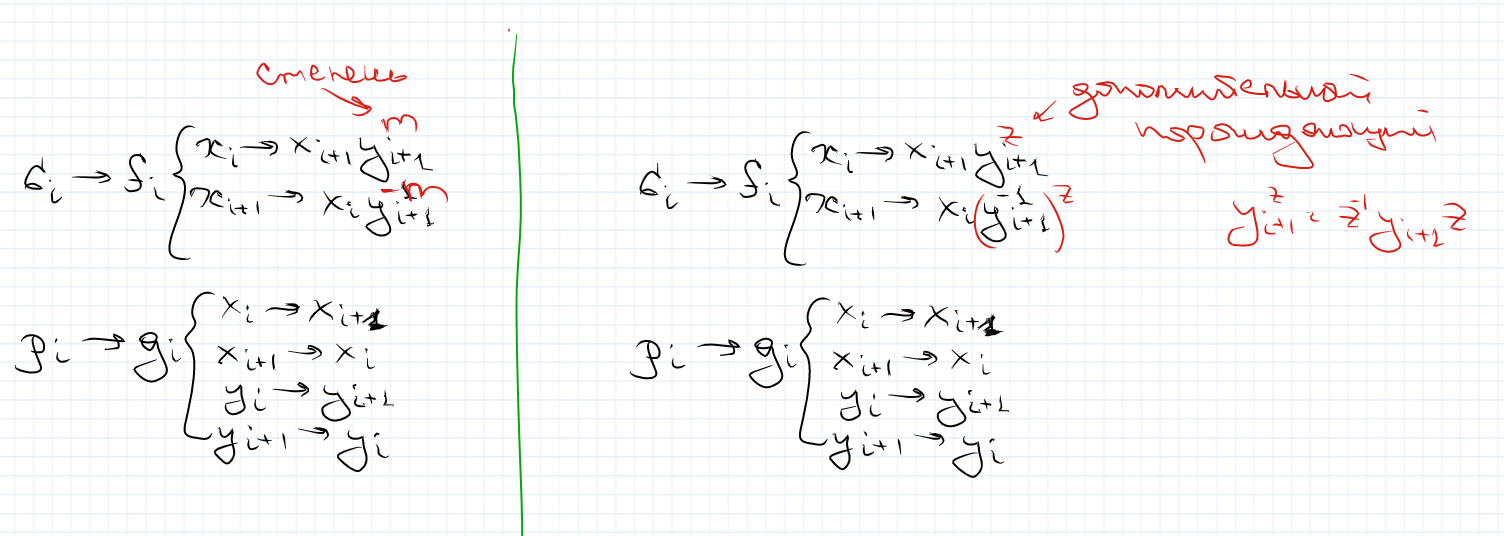
\includegraphics[width=110mm]{variant1.png}
     \item 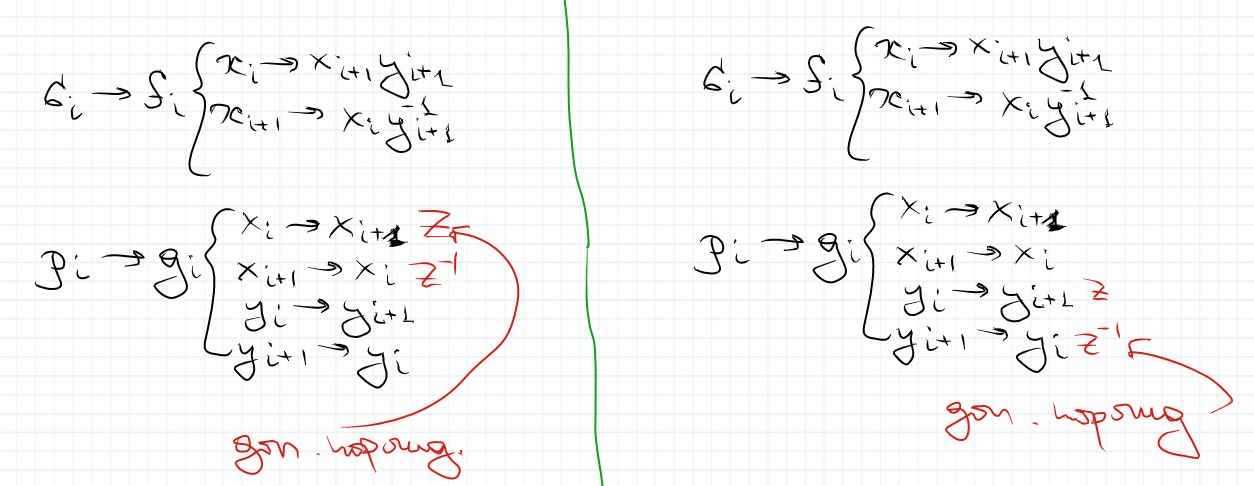
\includegraphics[width=110mm]{variant2.png}
      \item 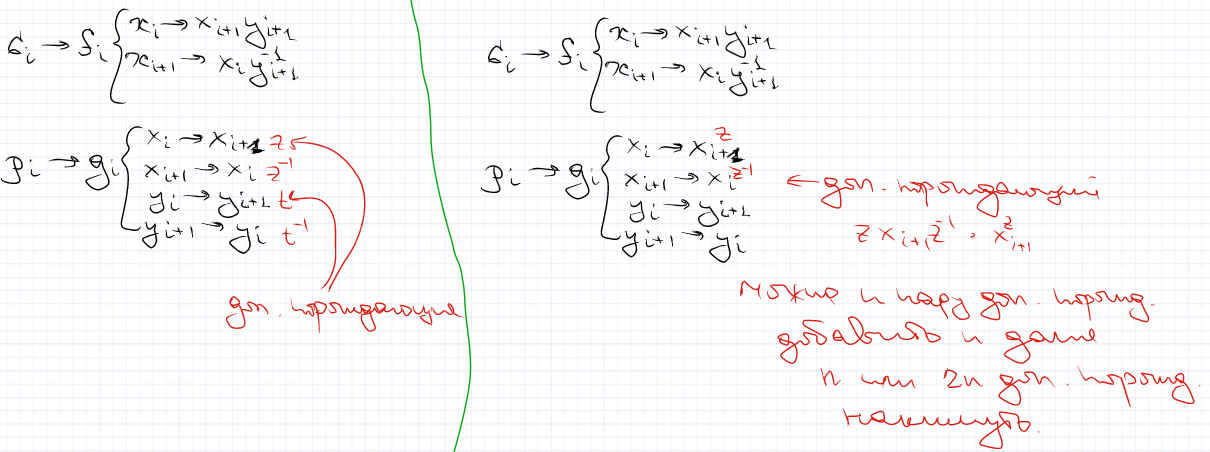
\includegraphics[width=110mm]{variant3.png}
\end{enumerate}
Most likely (up to my opinion) the map in the second line on the left is the representation. And this representation is better than the previous one (need to check).

Denote by $H_1$ the subgroup of $FVP_3=\langle a,b,c~|~[a,c]=1\rangle$ generated by the elements $a^3,b^2,c^3$. Find the intersection of $ker{\theta}$ with $H_1$. Is it trivial?

Denote by $H_2$ the subgroup of $FVP_3=\langle a,b,c~|~[a,c]=1\rangle$ generated by the elements $ac,b^2,c^3$. Find the intersection of $ker{\theta}$ with $H_2$. Is it trivial?

Denote by $H_3$ the subgroup of $FVP_3=\langle a,b,c~|~[a,c]=1\rangle$ generated by the elements $ac,b^2,a^3$. Find the intersection of $ker{\theta}$ with $H_3$. Is it trivial?

I choose $H_1,H_2,H_3$ in this way since the images of the elements which generate $H_1,H_2,H_3$ fix the elements $y_1,y_2,y_3$. 

Let $\alpha=(\rho_1\sigma_2)^6$, and let $x$ be an element from $VB_3$ (for example, $x=\rho_2$). Let $A$ be a subgroup in $VP_3$ generated by by two elements $\alpha$, $\beta=x^{-1}\alpha x$. Is it clear that this subgroup belongs to $ker(\theta)$. What can we say about this subgroup? Is it free? Can we compare it with the whole group $ker(\theta)$?

Can one reduce the dimension of the linear representation we got? I believe that it is possible and not difficult. The image of our linear representation acts on the vector space $V$ with the basis $e_1,e_2,e_3,q_1,q_2,q_3$. Look to the subspace $U$ generated by $e_1+e_2+e_3$, $q_1+q_2+q_3$. This subspace is invariant under $\theta(FVB_n)$. Look to the representation induced by $\theta$, which maps like $FVB_n\to GL(V/U)$.

Look to the kernel thinking about generators $\sigma_1, \sigma_2, \rho_1\sigma_1,\rho_2\sigma_2$. The first two generators move only the elements $x_1,x_2,x_3$, the second two generators move only the elements $y_1,y_2,y_3$.
\bibliographystyle{alpha}
\begin{thebibliography}{00}
\bibitem{problems}
R.~Fenn, D.~Ilyutko, L.~Kauffman, V.~Manturov, Unsolved problems in virtual knot theory and combinatorial knot theory, ArXiv:math/1409.2823.
\bibitem{BarBelDom}
V.~Bardakov, P.~Bellingeri, C.~Damiani, Unrestricted virtual braids, fused links and other quotients of virtual braid groups, J. Knot Theory Ramifications, V.~24, N.~12, 2015, 1550063.
\end{thebibliography}
\end{document}
